\typeout{Bewegingsherkenning met een smartphone}

\documentclass{article}
\usepackage[dutch]{babel}
\usepackage{ijcai11}
\usepackage{times}
\usepackage{tikz}
\usepackage{graphicx}
\usepackage{pgfplots}
\usepackage{rotating}

% voor deze packages: sudo apt-get install texlive-science
\usepackage[Algoritme]{algorithm}
\usepackage{algpseudocode}

\usepackage{subcaption}
%\usepackage{latexsym}  %optional

\title{Bewegingsherkenning met een smartphone}
\author{Arne De Brabandere\\
	arne.debrabandere@student.kuleuven.be
    \And
    Menno Keustermans\\
    menno.keustermans@student.kuleuven.be}
    
\tikzset{
    vertex/.style = {
        circle,
        fill            = black,
        outer sep = 2pt,
        inner sep = 1pt,
    }
}

\begin{document}

\maketitle

\begin{abstract}

Bewegingsherkenning is een belangrijke doelstelling van `context aware computing'. Uit de metingen van de accelerometer en gyroscoop van een smartphone kan de activiteit van de gebruiker bepaald worden. In het eerste deel van ons onderzoek hebben we gezocht naar een model om afzonderlijke activiteiten te herkennen. Het nauwkeurigste model werd gevonden met de classificatiemethode Random Forest met een accuraatheid van 93\%. Vervolgens hebben we dit model gebruikt om een sequentie van verschillende bewegingen te evalueren. Het algoritme dat we hiervoor ontwikkeld hebben, knipt de sequentie in opeenvolgende tijdsvensters van x aantal seconden die ook met een bepaald percentage kunnen overlappen. Uit experimenten bleek dat hiervoor een tijdsvenstergrootte van vier tot zes seconden met een overlapping van 75\% het nauwkeurigst is.

\end{abstract}

\section{Introductie}


\subsubsection{Geralateerd werk}
%TODO situering van het werk + bijdragen:
% - waarom bewegingen herkennen? (extra bronnen gebruiken
% - waarom met smartphones?
% - korte uitleg over onderzoek dat al gedaan is hierover voor afzonderlijke activiteiten (zie papers van literatuurstudie)
% - uitleg over eigen bijdrage: (1) van model om afzonderlijke activiteiten te herkennen naar algoritme om sequenties van activiteiten te herkennen (+ duidelijk zeggen wat we met afzondelijke activiteiten en sequenties bedoelen)



% bij 2 secties telkens "data collectie" + "data verwerking" + leermethodes + experimenten  +resultaten + conclusie

\section{Afzondelijke activiteiten}
\label{afzonderlijk}

Het eerste probleem is om van een gegeven reeks samples van de accelerometer en gyroscoop van een smartphone de activiteit van een persoon te bepalen. We veronderstellen hier dat telkens \'e\'en afzonderlijke activiteit gemeten wordt.

We willen tien verschillende activiteiten kunnen herkennen:
\begin{itemize}
\item wandelen,
\item lopen,
\item fietsen,
\item een trap opwandelen,
\item een trap afwandelen,
\item springen,
\item niets doen (zitten, liggen, staan),
\item een lift versnelt omhoog,
\item een lift versnelt omlaag,
\item tanden poetsen.
\end{itemize}

In bovenstaande lijst hebben we tanden poetsen als moeilijke activiteit toegevoegd. De beweging lijkt sterk op niets doen en zal waarschijnlijk minder goed te herkennen zijn.

Merk op dat we in plaats van de activeiten `lift naar boven of beneden nemen' enkel de versnelling van een lift naar boven of beneden in de lijst opnemen. Een lift naar boven nemen bevat dus de volgende activiteiten: lift versnelt omhoog~--~niets doen~--~lift versnelt omlaag. Het feit dat deze activiteiten ook `niets doen' bevatten, is de verklaring waarom we alleen de versnelling van een lift herkennen.
\\~\\
Het proces om de afzonderlijke activiteiten te herkennen verloopt in drie stappen. De eerste stap bestaat uit het verzamelen van de gegevens. Hiervoor meten we de versnellingen van de verschillende activiteiten. Als tweede stap worden features berekend uit de verzamelde gegevens. Deze zijn nodig om in de laatste stap modellen te leren met behulp van classificatiemethodes. Als criterium om de verschillende modellen te vergelijken, gebruiken we de accuraatheid als percentage van het aantal juiste geclassificeerde samples ten op zichte van het totaal aantal samples met behulp van cross-validatie.

%TODO ook motivatie (waarom classificatiemethodes)

\subsection{Gegevensverzameling}

Alle gegevens werden opgemeten door de MotionTracker tool. %TODO verwijzing met voetnoot: geschreven door ...
Dit is een Android-applicatie die de versnelling en rotatie (respectievelijk gemeten door de accelerometer en gyroscoop van de smartphone) samplet aan 50Hz.  Als uitvoer geeft de applicatie een .log-bestand met de gemeten versnellingen (in de x-as, y-as en z-as; de z-as is evenwijdig met de gravitatie) en rotaties (in quaternion notatie) met bijhorende timestamps.

Voor elke meting werd de applicatie gestart alvorens de smartphone in de broekzak gestopt werd en gestopt na het uithalen. Daarom bevat het begin en einde van elke meting enkele seconden die niet tot de gemeten activiteit horen. Om het fout labelen te vermijden, werd na elke meting een stuk van de start en het einde van het .log-bestand weggeknipt, zodat elke meting exact \'e\'en activiteit bevat van vier tot twintig seconden lang. 

Op deze manier hebben we voor elke activiteit 22 metingen verzameld, opgemeten door twee verschillende personen. Om voldoende variatie te hebben, gebeurden de metingen op verschillende dagen. Ook hebben we ervoor gezorgd dat we niet telkens dezelfde broek droegen, aangezien de gemeten versnelling kan vari\"eren in verschillende broekzakken. Na elke meting werd het resulterende .log-bestand geknipt en gelabeld met de juiste activiteit.

%TODO figuur met verschillende activiteiten

\subsection{Gegevensverwerking: features berekenen}

Voor we classificatiemethodes kunnen gebruiken, moeten we eerst features berekenen. Dit zijn parameters die we uit de samples van de accelerometer en gyroscoop kunnen halen. Om de verschillende features te berekenen, maken we gebruik van de MotionFingerprint tool. %TODO verwijzing naar tool 


%TODO uitleggen waarom we features berekenen

MotionFingerprint berekent in totaal 134 features\footnote{Het aantal features is afhankelijk van de instellingen van de tool.} verdeeld onder vier soorten:
\begin{itemize}
\item \textit{Statistische features:}
 dit zijn gemiddelde, standaardafwijking van zowel z- als xy-versnellingen en vermogen. En correlatie tussen z- en xy-versnelling,
 
\item \textit{Fourier transformatie:} deze worden berekend in het frequentie domein van de metingen, zoals amplitudes volgens de verschillende assen,

\item \textit{Wavelet transformatie:} \textbf{TODO}, %TODO

\item \textit{Hidden Markov models:} log-likelihood voor het model van elke activiteit.
\end{itemize}

%TODO uitleggen dat we verder voor de classificatiemethodes telkens 16 metingen gebruiken en dat we de andere 8 apart houden om HMM modellen te leren!

Na het berekenen van de features hebben we voor elke meting een set van parameters. Elke set vormt een instantie van de training set om een model te leren.

\subsubsection{Feature selectie}
%Waarom
Tussen de verschillende soorten features is er verschil in berekeningstijd en hoeveelheid informatie. Zo kunnen statistische features in het algemeen tegen een lagere kost berekend worden ten op zichte van Fourier transformatie features. In sommige toepassingen (zoals smartphone applicaties) kan het daarom interessant zijn om slechts een deel van het totaal aantal features te berekenen en juist diegene die de meeste informatie bevatten.

%Voorgestelde Oplossing
Met behulp van feature selectie onderzoeken we hoeveel features van het totaal aantal features van elke soort nodig zijn om een redelijke accuraatheid te behalen. Om de features met de meeste informatie te vinden, maken we gebruik van Weka's \emph{InfoGainAttributeEval} klasse. %TODO voetnoot naar weka informatie gain
 Deze klasse evalueert de waarde van elke feature met behulp van information gain.

%Evaluatie
Om vervolgens de geselecteerde features te evalueren maken we gebruik van dubbele cross-validatie. Bij de eerste cross-validatie (10-fold) wordt de gegevensset telkens verdeeld in een training en test set. Voor elke training set selecteren we de beste features met het proces dat hierboven werd beschreven, gebruik makend van een tweede cross-validatie (2-fold). Met de geselecteerde features wordt een model opgesteld met behulp van de Random Forest classificatiemethode in Weka. Het gevonden model wordt uiteindelijk ge\"evalueerd op de test set van de eerste cross-validatie.
	
%Resultaten
In figuur~\ref{fig:1} worden de resulaten voor de verschillende soorten features getoond. We zien dat we met enkel de statistische features al een accuraatheid van 90\% behalen. Zelfs met de helft van de features kan het model al met een accuraatheid van 80\% activiteit voorspellen. We stellen vast dat van het grote aantal Fourier tranformatie features slechts een tiental nodig zijn om een nauwkeurigheid van 80\% te bekomen. Wavelet transformatie features lijken minder goed te werken met slechts 70\% accuraatheid. Tenslotte merken we in de laatste grafiek op dat de Hidden Markov Models enkel degelijk werken wanneer alle features gebruikt worden.

\begin{figure}[htb]
\centering

  \begin{subfigure}[b]{.49\linewidth}
    \centering
    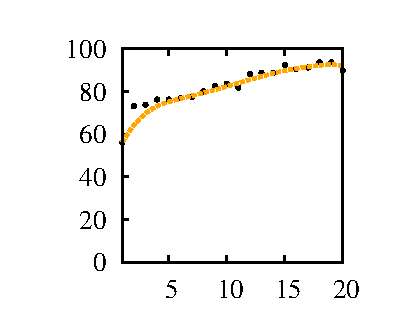
\includegraphics[width=0.99\textwidth]{figures/StatisticFeatures}
    \caption{Statistische features}\label{fig:1a}
  \end{subfigure}% 
  \begin{subfigure}[b]{.49\linewidth}
    \centering
    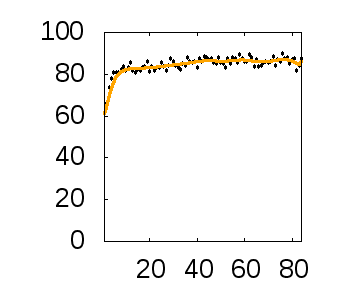
\includegraphics[width=.99\textwidth]{figures/FFTFeatures}
    \caption{FFT features}\label{fig:1b}
  \end{subfigure} \\
  \begin{subfigure}[b]{.49\linewidth}
    \centering
    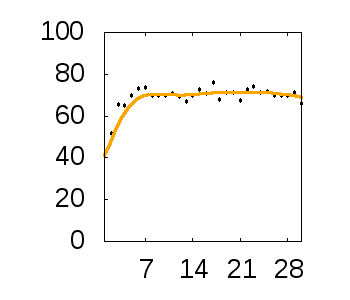
\includegraphics[width=.99\textwidth]{figures/DWTFeatures}
    \caption{Wavelet features}\label{fig:1c}
  \end{subfigure}
  \begin{subfigure}[b]{.49\linewidth}
    \centering
    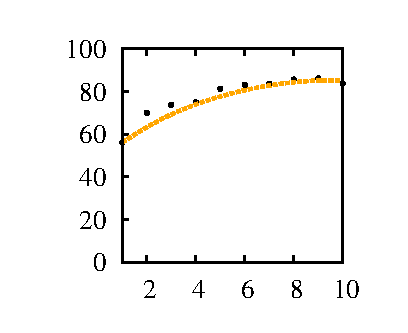
\includegraphics[width=.99\textwidth]{figures/HMMFeatures}
    \caption{HMM features}\label{fig:1e}
  \end{subfigure} \\
  

  \caption{Resultaten van het feature selectie experiment: op de x-as wordt steeds het aantal features van elke soort features geplot en op de y-as de accuraatheid (in percentages) van het model dat door Random Forest geleerd werd.}\label{fig:1}
\end{figure}

Voor de rest van het onderzoek wordt gebruik gemaakt van de volledige set features.



\subsection{Classificatiemethodes}

We gebruiken classificatiemethodes om een model te zoeken om afzonderlijke activiteiten te herkennen. We vergelijken enkele veel voorkomende methodes: beslissingsbomen, Random Forest, k-Nearest Neighbours, Naive Bayes en Support Vector Machines. De methodes leren telkens een model uit de instanties met de hierboven beschreven features voor de verschillende activiteiten. Hieronder wordt kort de werking van de vernoemde methodes beschreven:

\begin{itemize}
\item \textit{Beslissingsbomen} zijn bomen waarvan de interne knopen features voorstellen en de bladknopen \'e\'en (of meerdere) labels bevatten. Een tak in de boom stelt een test voor op de feature van de knoop waaruit de tak vertrekt. Om een nieuwe instantie te classificeren worden de juiste takken gevolgd tot in een bepaalde bladknoop. De instantie wordt dan geclassificeerd als het label in die bladknoop.
\item \textit{Random Forests} zijn combinaties van beslissingsbomen met een willekeurig deel van de trainingset en een willekeurig deel van de features. Bij de classificatie van een nieuwe instantie `stemt' elke boom op een label. De instantie krijgt vervolgens het label met de meeste stemmen.
\item \textit{k-Nearest Neighbours} classificeert nieuwe instanties door te zoeken naar de k dichtstbijzijnde instanties in de trainingset. Dit zijn de instanties waarvan de waarden voor de features het dichtst bij die van de te classificeren instantie ligt. Hieruit wordt het meest voorkomende label gekozen.
\item \textit{Naive Bayes} is een probabilistische classifier die gebruik maakt van voorwaardelijke kansen. De kans op een label $C$ met gegeven waarden voor de features $\mathbf{F}=(F_1, ..., F_n)$ wordt berekend als $P(C|\mathbf{F}) = { P(\mathbf{F}|C) P(C) \over P(\mathbf{F}) }$ waarin $P(\mathbf{F}|C)$, $P(C)$ en $P(\mathbf{F})$ uit de trainingset kunnen berekend worden. Bij het classificeren wordt het label met de grootste kans gekozen.
\item \textit{Support Vector Machines} beschouwt de features als een multidimensionele ruimte. De instanties zijn dan punten in de featureruimte. Bij het leren worden de instanties lineair van elkaar gescheiden door hypervlakken, zodat de instanties aan de ene kant van het vlak een ander label hebben dan die aan de andere kant. Wanneer de instanties niet lineair te scheiden zijn, worden ze getransformeerd met een \textit{kernel functie}. We gebruiken hier LibSVM, %TODO bron
waarbij binaire (\'e\'en-tegen-\'e\'en) classificatie gedaan wordt: elk hypervlak scheidt de instanties van 2 verschillende labels. Een nieuwe instantie wordt geclassificeerd door elke binaire classificatie als een stem voor een label te beschouwen. Het label met het grootste aantal stemmen wordt gekozen.
\end{itemize}

\subsection{Experimenten en resultaten}
\label{afzonderlijk:experimenten}

Om de methodes te evalueren, maken we gebruik van de Weka Machine Learning Toolkit. %TODO bronvermelding
Die bevat classifiers die de hierboven vermelde methodes implementeren. Voor beslissingsbomen maken we gebruik van de J48 classifier, een implementatie van het C4.5 algoritme. %TODO bronvermelding
Verder gebruiken we IBk voor k-Nearest Neighbours en LibSVM voor Support Vector Machines.

De evaluatie gebeurt met 10-fold cross-validatie. Hierbij worden de instanties op 10 verschillende manieren opgesplitst zodat telkens 90\% van de instanties als trainingset wordt gebruikt om een model uit te leren. Op de overige 10\% wordt het model ge\"evalueerd. De accuraatheid van elke methode wordt dan berekend als het gemiddelde percentage van correct geclassificeerde instanties in de verschillende testsets.

\begin{figure}
\centering
\begin{tikzpicture}
\begin{axis}[
    ybar,
    xtick=data,
    ymin=0,
    xticklabels from table={Data/methodes.dat}{methode},
    xticklabel style={align=center},
    nodes near coords,
    ylabel={Accuraatheid (\%)}
]

\addplot table [
    x=xpos,
    y=accuraatheid
] {Data/methodes.dat};

\end{axis}
\end{tikzpicture}
\caption{Accuraatheid van classificatiemethodes}
\label{fig:methodes}
\end{figure}

In figuur \ref{fig:methodes}
wordt de accuraatheid van de verschillende classificatiemethodes vergeleken. We zien dat Random Forest de hoogste accuraatheid geeft voor de metingen. Ook J48 geeft een goede accuraatheid. De hogere accuraatheid van Random Forest ten opzichte van beslissingsbomen is te verklaren door het feit dat Random Forest minder kans op overfitting heeft.~\cite{breiman:randomforests} Naive Bayes lijkt ook goed te werken, terwijl met IBk en vooral LibSVM een lagere accuraatheid bereikt wordt. De accuraatheid van de methodes kan echter wel verbeterd worden door de parameters de optimaliseren.

\begin{figure*}
\begin{center}
{ \footnotesize
\begin{tabular}{ c | c | c | c | c | c | c | c | c | c | l }
     \begin{sideways} Wandelen       \end{sideways}
  &  \begin{sideways} Lopen          \end{sideways} 
  &  \begin{sideways} Fietsen        \end{sideways} 
  &  \begin{sideways} Trap op        \end{sideways} 
  &  \begin{sideways} Trap af        \end{sideways} 
  &  \begin{sideways} Springen       \end{sideways} 
  &  \begin{sideways} Niets doen     \end{sideways} 
  &  \begin{sideways} Lift omhoog    \end{sideways} 
  &  \begin{sideways} Lift omlaag    \end{sideways} 
  &  \begin{sideways} Tanden poetsen \end{sideways} 
  &  $\leftarrow$ \parbox[b]{1.8cm}{geclassificeerd\\als} \\   \hline
 16 &    &    &    &    &    &    &    &    &    & Wandelen           \\   \hline
    & 16 &    &    &    &    &    &    &    &    & Lopen              \\   \hline
    &    & 16 &    &    &    &    &    &    &    & Fietsen            \\   \hline
    &    &    & 15 &  1 &    &    &    &    &    & Trap op            \\   \hline
    &    &    &    & 16 &    &    &    &    &    & Trap af            \\   \hline
    &    &    &    &    & 16 &    &    &    &    & Springen           \\   \hline
    &    &    &    &    &    & 14 &    &    &  2 & Niets doen         \\   \hline
    &    &    &    &    &    &    & 10 &  6 &    & Lift omhoog        \\   \hline
    &    &    &    &    &    &    &  1 & 15 &    & Lift omlaag        \\   \hline
    &    &    &    &    &    &    &    &    & 16 & Tanden poetsen
\end{tabular}
}
\end{center}
\caption{Confusion matrix voor Random Forest}
\label{fig:confusionmatrix}
\end{figure*}

Voor het model dat door Random Forest geleerd wordt, hebben we in figuur \ref{fig:confusionmatrix} een confusion-matrix geplot. Het valt op dat activiteiten met grote versnellingen -- wandelen, lopen, fietsen en springen -- goed te herkennen zijn. Alle metingen voor deze activiteiten worden immers correct geclassificeerd door het model. Niets doen, lift omhoog/omlaag en tanden poetsen hebben kleinere versnellingen dan de andere activiteiten. We zien dat 2 metingen van niets doen als tanden poetsen worden geclassificeerd. Ook lift omhoog en omlaag worden gemakkelijk met elkaar verward. Omwille van de kleine versnellingen zijn de verschillen tussen de activiteiten subtieler, wat een verklaring kan zijn waarom deze activiteiten moeilijker te herkennen zijn.





\section{Sequenties van activiteiten}

Bij het herkennen van afzonderlijke activiteiten bevat elke meting exact \'e\'en activiteit. De classificatiemethodes die we hiervoor gebruiken zijn dus niet rechtstreeks toepasbaar op metingen waarin verschillende activiteiten na elkaar gebeuren. Daarom gaan we op zoek naar een methode om voor een sequentie van activiteiten te bepalen welke activiteiten daarin gedaan worden en wanneer.

\subsection{Gegevensverzameling}

Met behulp van de MotionTracker applicatie werd opnieuw de versnelling en rotatie gemeten, maar nu van meerdere activiteiten na elkaar. In totaal zijn vier sequenties van elk ongeveer drie minuten lang opgemeten: twee verschillende combinaties van activiteiten, telkens door twee personen opgemeten. De ene combinatie bevat de activiteiten wandelen, trap op en af, niets doen, lopen en springen. De andere bevat wandelen, trap op en af, niets doen en lift omhoog en omlaag. Omdat lift versnellingen moeilijk van elkaar te onderscheiden zijn door het model voor afzonderlijke activiteiten (zie sectie~\ref{afzonderlijk:experimenten}), is de tweede combinatie moeilijker te herkennen dan de eerste.

Om de metingen te evalueren, werd elke sequentie gelabeld met behulp van een .csv-bestand. Dit bestand bevat de start- en eindtijden van de verschillende activiteiten in de bijhorende meting. De delen die niet gelabeld werden, beschouwen we als ruis. Het gaat om periodes met activiteiten die niet tot de tien activiteiten behoren die we kunnen herkennen. De smartphone in de broekzak stoppen is hier een voorbeeld van.

\subsection{Gegevensverwerking}

Aangezien de modellen voor afzonderlijke activiteiten niet rechtstreeks kunnen toegepast worden op sequenties, moeten de sequenties geknipt worden in delen die wel \'e\'en activiteit bevatten. We doen dit door de sequenties in tijdsvensters op te splitsen. De vensters hebben een lengte van enkele seconden en kunnen overlappen opdat er meer kans is dat een venster \'e\'en activiteit bevat. We defini\"eren een overlapping als het percentage van de lengte van een tijdsvenster dat ook tot het eerst volgende tijdsvenster hoort. In figuur \ref{fig:overlap} wordt ge\"illustreerd wat een overlapping van bijvoorbeeld 75\% betekent.

\begin{figure}
\begin{center}
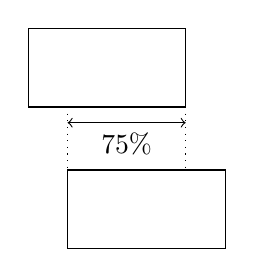
\begin{tikzpicture}
\draw (0.5,-0.8) -- (2.5,-0.8) -- (2.5,0.2) -- (0.5,0.2) -- (0.5,-0.8);
\draw (0,1) -- (2,1) -- (2,2) -- (0,2) -- (0,1);

\draw [<->] (0.5,0.8) -- node[below] {75\%} (2,0.8);
\draw [dotted] (0.5,1) -- (0.5,0.2);
\draw [dotted] (2,1) -- (2,0.2);
\end{tikzpicture}
\end{center}
\caption{Tijdsvensters met een overlapping van 75\%}
\label{fig:overlap}
\end{figure}

\subsection{Algoritme}

Bij het voorspellen van de activiteiten van een sequentie maken we gebruik van de tijdsvensters. We beschrijven een algoritme waarmee voor elke halve seconde van een sequentie een voorspelling kan gemaakt worden voor de activiteit die daarin gebeurde.

Het algoritme heeft drie parameters nodig: de lengte van de tijdsvensters in seconden, de overlapping ervan ials een percentage en een ruis cutoff kans. De laatste parameter wordt verder verduidelijkt. In sectie~\ref{sequenties:experimenten} worden experimenten uitgevoerd om de waarden voor deze parameters te kiezen zodat de voorspellingen van het algoritme zo correct mogelijk zijn.

Voor de pseudo-code van het algoritme verwijzen we naar Algoritme~\ref{alg:sequentie}. De eerste stap bestaat uit het splitsen van de sequentie in tijdsvensters met de gegeven lengte en overlapping. Vervolgens wordt voor elk deel van een halve seconde lang van de sequentie gecontroleerd welke tijdsvensters dat deel bevatten. Deze vensters zijn samen met de ruis cutoff kans de parameters van Algoritme~\ref{alg:deel} om de activiteit van het deel van de sequentie te bepalen. Hierbij wordt voor elk venster een voorspelling gemaakt met behulp van een model om afzonderlijke activiteiten te classificeren. In sectie~\ref{afzonderlijk} bleek Random Forest het best te werken. Daarom gebruiken we hier het model dat door deze methode geleerd werd. Voor elk venster laten we ook de kans berekenen dat het voorspelde label correct is. Bij Random Forest wordt deze kans bepaald als het percentage van de bomen die dat label voorspellen. %TODO klopt dit? want ik vind er niet onmiddellijk iets over...
Als minstens twee vensters met het deel van de sequentie overlappen, houdt het algoritme geen rekening met de kansen wanneer de voorspelde labels van de vensters gelijk zijn. In dat geval wordt als voorspelling het label van de tijdsvensters voorspeld. Anders controleert het algoritme of er een label is met een kans groter dan de ruis cutoff kans. Indien dat zo is, wordt voor het deel van de sequentie het label met de grootste kans als activiteit voorspeld. Wanneer alle kansen onder de ruis cutoff kans liggen, zal de voorspelling `Ruis' zijn.

\begin{algorithm}
  \caption{Activiteiten van een sequentie (met start en eind timestamp in seconden) voorspellen door als uitvoer een lijst terug te geven met voor elke halve seconde de voorspelde activiteit}
  \label{alg:sequentie}
  \begin{algorithmic}[0]
    \State \textbf{Parameters:}\\
    $lengte$ van de tijdsvensters (in seconden) \\
    $overlapping$ van de tijdsvensters (percentage) \\
    $cutoff$ voor ruis (kans) \\
    \State Splits de sequentie op in tijdsvensters met gegeven $lengte$ en $overlapping$ \\
    \For{$t$ = $start$; $t$ $\le$ $einde$; $t$ += $0.5s$}
      \State $vensters$ = tijdsvensters die $t$ en $t+0.5s$ bevatten
      \State $voorspellingen$[$t$] = \textsc{activiteit}($vensters,cutoff$) \\
      \Comment{zie algoritme \ref{alg:deel}}
    \EndFor \\
    \State \textbf{return} $voorspellingen$
  \end{algorithmic}
\end{algorithm}

\begin{algorithm}
  \caption{Activiteit van een deel van een sequentie bepalen, met een gegeven lijst van tijdsvensters en een ruis cutoff kans}
  \label{alg:deel}
  \begin{algorithmic}[0]
    \Procedure{activiteit}{$vensters, cutoff$}
      \State $labels$ = voorspelde activiteiten voor $vensters$ 
      \State $kansen$ = kansen voor de $labels$ \\
      \Comment{berekend door model van Random Forest} \\
      \If{aantal $vensters$ $\ge$ 2 \textbf{and} alle $labels$ gelijk}
        \State \textbf{return} $labels$[$0$]
      \Else
        \If{$kansen$[$i$] $>$ $cutoff$ voor een $i$}
          \State \textbf{return} $labels$[$i$] met $kansen$[$i$] maximaal
        \Else
          \State \textbf{return} `Ruis'
        \EndIf
      \EndIf
    \EndProcedure
  \end{algorithmic}
\end{algorithm}

%TODO algoritme uitleggen + hierbij ook uitleg over ruis-cutoff

\subsection{Experimenten en resultaten}
\label{sequenties:experimenten}

%TODO
% - hoe gebeurt de evaluatie?
% - accuraatheid plotten in functie van grootte van tijdsvensters en overlap + tijdsvensters vergelijken + iets over ruis cut-off
%   ==> hypothese (waarschijnlijk 4sec en 3/4 overlap, omwille van activiteit lift versnelt omhoog/omlaag)
% - bespreking van resultaten: komt dit overeen met de hypothese?

\section{Conclusie}

%TODO voor afzonderlijke activiteiten EN (?) voor sequenties

\section{Verder werk}

%TODO misschien wat er zou gebeuren als hetzelfde zou gedaan worden voor meer metingen? (bvb. wandelen, lopen, ... accurater)




%TODO bronvermelding!

%% The file named.bst is a bibliography style file for BibTeX 0.99c
\bibliographystyle{named}
\bibliography{paper}

\end{document}

